\documentclass[12pt]{article}
\usepackage[T1]{fontenc}
\usepackage[margin=2cm]{geometry}

\usepackage{amssymb}
\usepackage{amsmath}
\usepackage{tcolorbox}
\usepackage{xcolor}
\usepackage{framed}
\usepackage{euscript}
\usepackage{float}

\usepackage{verbatim}
\usepackage{mathrsfs}
\usepackage{graphicx}
\usepackage{multicol}

\usepackage{bbm,txfonts}
\usepackage{float}


\usepackage{titletoc}
\usepackage{tikz}
\usepackage{xspace}

\usepackage{enumitem}

\newcommand{\answer}{\vspace*{4pt} \noindent{\bf Solution: }}

\newcommand{\bb}[1]{\mathbb{#1}}
\renewcommand{\v}[1]{\boldsymbol{#1}}
\newcommand{\m}[1]{\mathbf{#1}}
\renewcommand{\c}[1]{\mathcal{#1}}
\usepackage{upquote}


\renewcommand{\tilde}{\widetilde}
\newcommand{\halmos}{\vspace{3mm} \hfill \mbox{$\Box$}}

\newcommand{\Var}{\mathbb{V}\mathrm{ar}}
\newcommand{\var}{\Var}

\newcommand{\Cov}{\mathbb{C}\mathrm{ov}}
\newcommand{\cov}{\Cov}

\renewcommand{\epsilon}{\varepsilon}
\renewcommand{\rho}{\varrho}
\renewcommand{\log}{\ln}
\renewcommand{\hat}{\widehat}

\newcommand{\iid}{\text{iid }}


% Bernoulli distribution
\newcommand{\Ber}{{\sf Ber}}
\newcommand{\ber}{\Ber}

% Binomial distribution
\newcommand{\Bin}{{\sf Bin}}
\newcommand{\bin}{\Bin}

% Cauchy distribution
\newcommand{\Cauchy}{{\sf Cauchy}}

% Negative binomial distribution
\newcommand{\NegBin}{{\sf NegBin}}

% Multinomial distribution
\newcommand{\Mnom}{{\sf Mnom}}
\newcommand{\mnom}{\Mnom}

% Geometric distribution
\newcommand{\Geo}{{\sf Geom}}
\newcommand{\geo}{\Geo}
\newcommand{\Geom}{\Geo}
\newcommand{\geom}{\Geo}
\newcommand{\G}{\Geo}

% Hypergeometric distribution
\newcommand{\Hyp}{{\sf Hyp}}

% Poisson distribution
\newcommand{\Poi}{{\sf Poi}}
\newcommand{\poi}{\Poi}
\newcommand{\Po}{\Poi}
\newcommand{\po}{\Poi}

% Uniform distribution (continuous)
\newcommand{\U}{\EuScript{U}}

% Exponential distribution
\newcommand{\Ex}{{\sf Exp}}
\newcommand{\ex}{\Ex}

% Normal / Gaussian distribution
\newcommand{\Nor}{\EuScript{N}}
\newcommand{\nor}{\Nor}

% Pareto distribution
\newcommand{\Pareto}{{\sf Pareto}}
\newcommand{\pareto}{\Pareto}

% Negative hypergeometric distribution
\newcommand{\NegHyp}{{\sf NegHyp}}

% Student's t distribution
\newcommand{\Student}{{\sf t}}
\newcommand{\student}{\Student}

% Gamma distribution
\newcommand{\Gam}{{\sf Gamma}}
\newcommand{\gam}{\Gam}

% Discrete uniform distribution
\newcommand{\DU}{{\sf DU}}

% Generic distribution
\newcommand{\Dist}{{\sf Dist}}

\newcommand{\Em}{{\mathbb E}}  % expectation
\newcommand{\Pm}{{\mathbb P}}  % probability measure
\newcommand{\R}{{\mathbb R}}

\newcommand{\gvn}{\,|\,}  % conditional (given)

\newcommand{\e}{\mathrm{e}} %Euler's e

\newcommand{\ds}{\displaystyle}

\newcommand{\di}{\mathrm{d}}  % use for differential symbol


\newcommand{\approxsim}{\stackrel{\mathrm{approx.}}{\sim}}

\newcommand{\iidsim}{\stackrel{\mathrm{iid}}{\sim}}
\newcommand{\simiid}{\iidsim}
\newcommand{\simiidt}{{\:{\sim}_{\mathrm{iid}}\:}}

%% Correlation
\newcommand{\Corr}{\mathrm{Corr}}
\newcommand{\corr}{\Corr}


\usepackage{cprotect}
\RequirePackage[formats]{listings}\RequirePackage{textcomp}

\lstnewenvironment{Pout}{%
  \lstset{backgroundcolor=\color{outcol},
  aboveskip= -2pt,  
  xleftmargin = 4pt,
  xrightmargin = 4pt,
  frame=single,
  upquote,
  framerule=1pt,
  basicstyle=\footnotesize\ttfamily,
  columns=fixed}}{}

%DK: See http://latexcolor.com/
\definecolor{applegreen}{rgb}{0.55, 0.41, 0.0}
\definecolor{gray1}{rgb}{0.98, 0.98, 0.98}
\definecolor{black}{rgb}{0, 0, 0}
\definecolor{cream}{rgb}{1.0, 0.99, 0.82}
\definecolor{islamicgreen}{rgb}{0.0, 0.56, 0.0}
\definecolor{vlgray}{gray}{0.9}
\definecolor{lgray}{gray}{0.7}
\definecolor{outcol}{gray}{0.9}

\tcbuselibrary{listings,skins,breakable,theorems}

\newenvironment{PC}{%
\tcblisting{breakable,listing only,colback=cream, enhanced, sharpish
corners,  boxrule=1pt,after, listing options =
   {language=Python,
  basicstyle=\footnotesize\ttfamily,        % the size of the fonts that are used for the code
  numbers=none,                   % where to put the line-numbers
%  numberstyle=\tiny\color{blue},  % the style that is used for the line-numbers
  xleftmargin=-10pt,
  aboveskip=-4pt,
  belowskip=-6pt,
  columns=fixed,
  basewidth=5pt,                     %separation of letters
%  stepnumber=1,                % the step between two line-numbers. If it's 1, each line will be numbered
%  numbersep=7pt,                  % how far the line-numbers are from the code
  backgroundcolor=\color{cream},  % choose the background color. You must add \usepackage{color}
  showspaces=false,               % show spaces adding particular underscores
  showstringspaces=false,         % underline spaces within strings
  showtabs=false,                 % show tabs within strings adding particular underscores
  %frame=single,                   % adds a frame around the code
  %frame=shadowbox,
  %rulecolor=\color{black},        % if not set, the frame-color may be changed on line-breaks within not-black text (e.g. comments (green here))
  tabsize=2,                     % sets default tabsize to 2 spaces
 % captionpos=b,                  % sets the caption-position to bottom
  breaklines=true,                % sets automatic line breaking
  breakatwhitespace=false,        % sets if automatic breaks should only happen at whitespace
  %title=\lstname,                 % show the filename of files included with \lstinputlisting;
                                  % also try caption instead of title
  keywordstyle=\color{blue},      % keyword style
  upquote,     % very important to get right quote for cut/paste
  commentstyle=\color{islamicgreen},   % comment style
  stringstyle=\color{red},      % string literal style
 % escapeinside={\%*}{*)},         % if you want to add a comment within your code
  morekeywords={*,...}
  			 }
    		}
    	}
{\endtcblisting}







\usepackage{fvextra}
\DefineVerbatimEnvironment{Code}{Verbatim}{
    fontsize=\footnotesize, % Adjust font size
    breaklines=true,        % Enable line wrapping
    breakanywhere=true      % Allow breaking anywhere
}

\begin{document}
\begin{center}

{\Large  {\bf Machine Learning (COMP7703)}

Table Tennis Project Plan - Semester 1, 2025.

\vspace{10pt}

{\large Volter Entoma}

{\large 44782711}
}
\end{center}

The 3D-PCA visualization of the data for different swing modes reveals that there is quite a lot of overlap between the different modes.
This suggests that the swing modes are not easily separable in the feature space, and that a more complex model may be needed to accurately predict the swing mode from the data.
For this project I propose the research question: \textit{are there any more styles of swings beyond the three predefined modes?}

For reference, the list of swing modes:

\begin{itemize}
    \item $test\_mode = 0$ (Swing in the air)
    \item $test\_mode = 1$ (Full power stroke)
    \item $test\_mode = 2$ (Stable stroke)
\end{itemize}

The 3D-PCA visualization of the data with different colors for different swing modes.
\begin{figure}[h!]
    \centering
    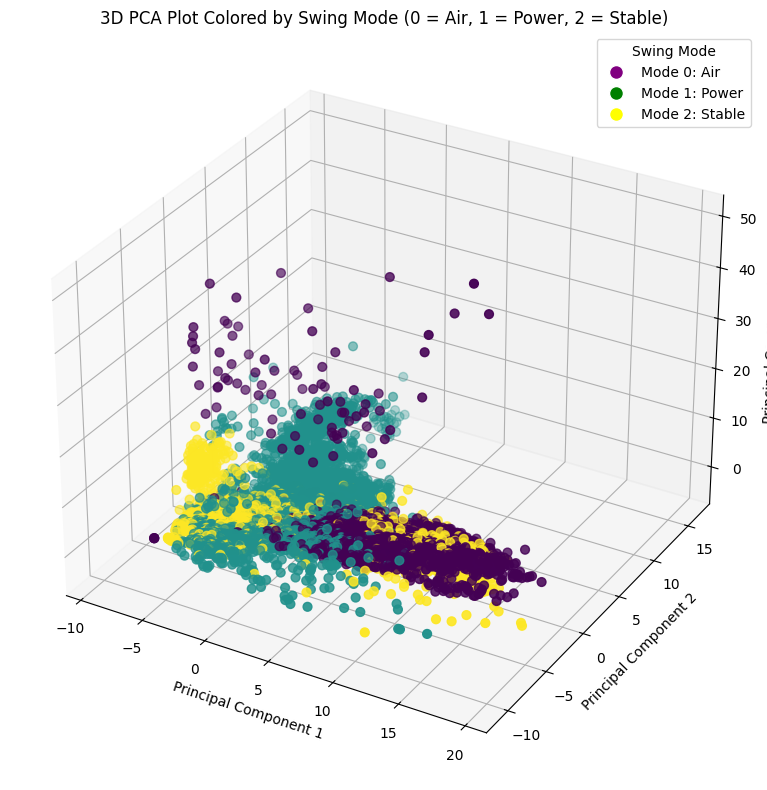
\includegraphics[width=0.6\textwidth]{3d_pca_swing_modes.png}
    \caption{3D-PCA visualization of the data with different colors for different swing modes.}
    \label{fig:3d_pca}
\end{figure}


I theorize that there are four more "intermediate" swing modes that are not explicitly defined in the dataset. These modes are, Air-Power, Air-Stable, Power-Stable, and Air-Power-Stable. These modes are not explicitly defined in the dataset, but are inferred from strong overlap of some data points from swing mode to another.

I ran a quick pilot test using unsupervised learning using KMeans clustering to see if it could classify the overlap between the different swing modes. The results are shown in the figure below.

\begin{figure}[h!]
    \centering
    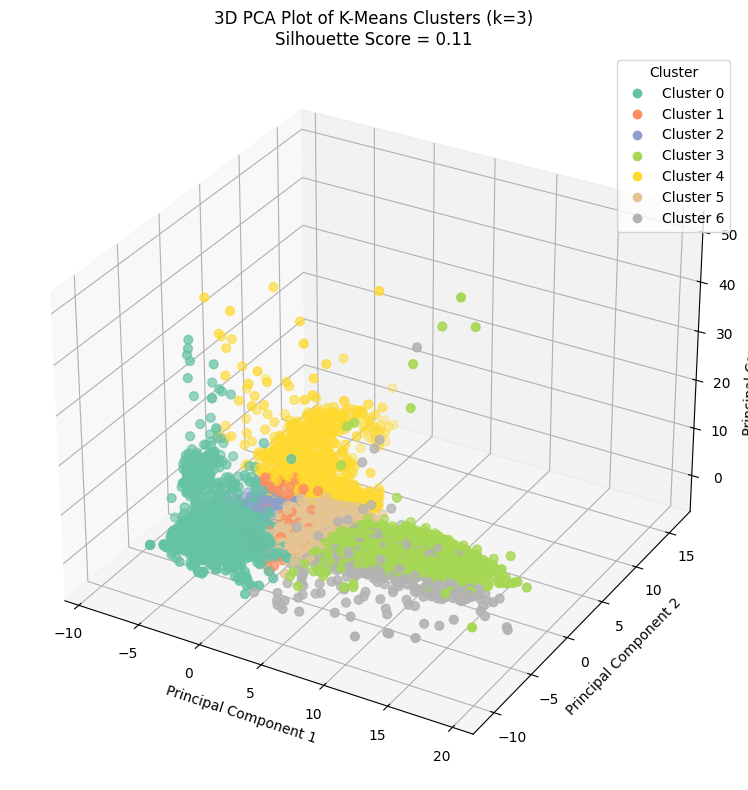
\includegraphics[width=0.6\textwidth]{3d_pca_kmean_clustering.png}
    \caption{KMeans clustering of the data.}
    \label{fig:kmeans}
\end{figure}

A quick look into the KMeans clustering results shows that the model was able to classify the data into 7 clusters. In particular, "Cluster 0" seems to correlate with the "Stable", "Cluster 6" with the "Air", and "Cluster 4" with the "Power" swing modes. 
The other clusters are not as clear, however they seem to correlate with the intermediate swing modes I proposed. 

While the original labels identify three swing types, the unsupervised analysis using 3D PCA and KMeans ($k=7$) reveals a more complex structure. Overlaps between modes suggest transitional forms, which align with the idea of intermediate swing styles. 
Although the silhouette score is quite low ($0.11$), indicating that the clusters are not well separated, a visual analysis of the clustering suggest that there are indeed more than three swing modes.

The question now is whether these clusters are latent structures or if they are artifacts of the clustering algorithm.

The confusion-matrix below shows the results of the KMeans clustering.

\begin{figure}[H]
    \centering
    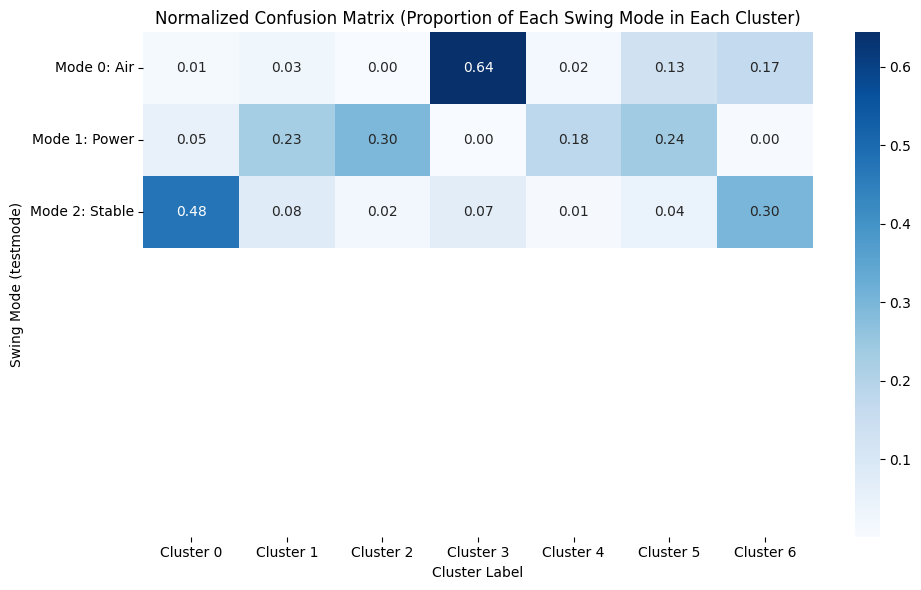
\includegraphics[width=0.6\textwidth]{normalized_confusion_matrix.png}
    \caption{Normalized confusion matrix of the KMeans clustering.}
    \label{fig:confusion_matrix}
\end{figure}

\textbf{Things-to-do:}
\\
\textbf{Cluster Stability Across Different Methods}\\
- Use different $k$ values to see if the clusters are stable across different $k$ values.\\
- Use different clustering methods (e.g., DBSCAN, Agglomerative Clustering) to see if the clusters are stable across different methods.\\
- Use different dimensionality reduction methods (though I'm not sure if this is a good idea) to see if the clusters are stable across different methods.\\

\vspace{20pt}

\newpage

\end{document}
